% =============================================================================
% P3D -- Privacy 2: poster (EN), style2 version
% Style of the P2A poster (_grupo/P2A/mainV3.tex): a0poster A1 portrait, UnB mark,
% green small-caps title, two columns with numbered blue headings, no boxes.
% Figures expected in out/: FigP1_EN.pdf, FigP3_EN.pdf (built from figuras/).
% The heat map (Figure 2) is a colored table written in this file.
% UnB mark: figuras/marca_unb.png. Content equals P3D_Privacidade2_Poster_EN.tex.
% =============================================================================
\documentclass[a1,portrait]{a0poster}
\usepackage[brazil,english]{babel}
\usepackage[utf8]{inputenc}
\usepackage[absolute]{textpos}
\usepackage{graphicx}
\usepackage{color}
\usepackage[table]{xcolor}
\usepackage{amsmath,amssymb}
\usepackage{booktabs}

\definecolor{DarkBlue}{rgb}{0.1,0.1,0.5}
\definecolor{Red}{rgb}{0.9,0.0,0.1}
\definecolor{DarkGreen}{rgb}{0.10,0.50,0.10}
\definecolor{exLine}{RGB}{23,54,93}

\let\Textsize\normalsize
\def\LHead#1{\noindent{\LARGE\color{DarkBlue} #1}\smallskip}
\def\Subhead#1{\noindent{\large\color{DarkBlue} #1}}
\newcommand{\quiteHuge}{\fontsize{55}{70}\selectfont}
\def\Title#1{\begin{center}\noindent{\quiteHuge\color{DarkGreen}#1}\end{center}}

\TPGrid[40mm,40mm]{23}{12}

\parindent=0pt
\parskip=0.5\baselineskip

\begin{document}
\large

\begin{textblock}{23}(0,0)
\centering

\includegraphics[width=18cm]{figuras/marca_unb.png}
\end{textblock}

\begin{textblock}{23}(0,0.5)
\Title{\textsc{PMBOK 8 on one page: principles, processes and tailored practice}}
\end{textblock}

\begin{textblock}{23}(0,1.1)
\begin{center}
  \parbox{0.8\textwidth}{
    \small
    \begin{center}
    \textbf{Authors:} Filipe Alves de Sousa and Members of the Recycling 1 Group\\
    \textbf{Course:} IT Project Management (GPTI) -- PPCA/CIC/UnB\\
    \textbf{Deliverable:} P3D | \textbf{Code:} 3p2 / 3R31
    \end{center}
  }
\end{center}
\end{textblock}

% ------------------------------- LEFT COLUMN ----------------------------------
\begin{textblock}{11}(0,2.0)

\LHead{1. Principles and tailoring}

Principles guide decisions; domains and Focus Areas organize the work; tailoring adjusts their application [5].

\begin{figure}[h!]
\centering
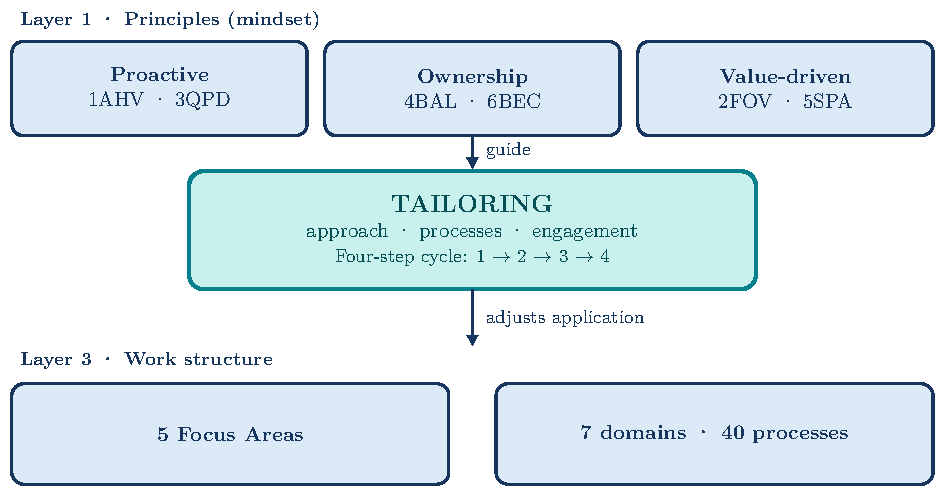
\includegraphics[width=\linewidth]{out/FigP1_EN.pdf}
\caption{Principles and tailoring.}
\end{figure}

\textbf{Five operations on processes:} add $\cdot$ modify $\cdot$ remove $\cdot$ blend $\cdot$ align. \textbf{Three objects of tailoring:} life cycle and development approach $\cdot$ processes $\cdot$ engagement [5].

\vspace{0.3cm}
\LHead{2. Map of 40 processes}

{\normalsize
\setlength{\tabcolsep}{4pt}
\renewcommand{\arraystretch}{1.3}
\noindent\begin{tabular*}{\linewidth}{@{\extracolsep{\fill}}lrrrrrr}
\hline
\textbf{Domain} & \textbf{IN} & \textbf{PL} & \textbf{EX} & \textbf{MC} & \textbf{CL} & \textbf{Total}\\
\hline
Governance & \cellcolor{exLine!9}1 & \cellcolor{exLine!18}2 & \cellcolor{exLine!27}3 & \cellcolor{exLine!18}2 & \cellcolor{exLine!9}1 & 9\\
Scope & 0 & \cellcolor{exLine!36}4 & 0 & \cellcolor{exLine!18}2 & 0 & 6\\
Schedule & 0 & \cellcolor{exLine!18}2 & 0 & \cellcolor{exLine!9}1 & 0 & 3\\
Finance & 0 & \cellcolor{exLine!27}3 & 0 & \cellcolor{exLine!9}1 & 0 & 4\\
Stakeholders & \cellcolor{exLine!9}1 & \cellcolor{exLine!18}2 & \cellcolor{exLine!18}2 & \cellcolor{exLine!18}2 & 0 & 7\\
Resources & 0 & \cellcolor{exLine!18}2 & \cellcolor{exLine!18}2 & \cellcolor{exLine!9}1 & 0 & 5\\
Risk & 0 & \cellcolor{exLine!36}4 & \cellcolor{exLine!9}1 & \cellcolor{exLine!9}1 & 0 & 6\\
\hline
\textbf{Total} & \textbf{2} & \textbf{19} & \textbf{8} & \textbf{10} & \textbf{1} & \textbf{40}\\
\hline
\end{tabular*}\par}

\vspace{0.2cm}
{\small \textbf{Legend:} IN Initiating $\cdot$ PL Planning $\cdot$ EX Executing $\cdot$ MC Monitoring and Controlling $\cdot$ CL Closing. Process count $\neq$ duration or importance of an area. \textit{Identify Stakeholders} is in Initiating (Guide Figure 2-32).}

\end{textblock}

% ------------------------------- RIGHT COLUMN ---------------------------------
\begin{textblock}{11}(12,2.0)

\LHead{3. Four domain concentrations}

\begin{figure}[h!]
\centering
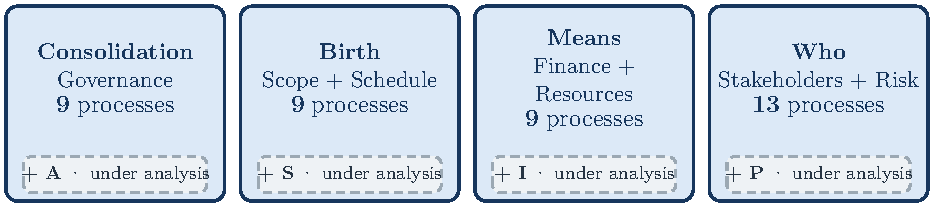
\includegraphics[width=\linewidth]{out/FigP3_EN.pdf}
\caption{Four domain concentrations.}
\end{figure}

\textbf{Reading notice:} the four concentrations and the A, S, I, and P labels are the \textbf{analytical grouping of this work}; the seven domains and their 40 processes are from PMBOK 8 [5].

\vspace{0.3cm}
\LHead{4. How to use this summary}

Select an initial approach, tailor it to the organization and project, and improve it continuously [5]. The map locates the 40 processes without prescribing a single sequence; process counts do not indicate duration or importance. PMBOK 8 does not describe digital twins. Studies of hybrid approaches [4, 6] help place tailoring decisions in context.

\vspace{0.3cm}
\LHead{5. Key references}

{\normalsize
[4] NOLL, J.; BEECHAM, S. How agile is hybrid agile? An analysis of the HELENA data. \textbf{PROFES 2019}, LNCS vol. 11915, pp. 341--349, 2019.

[5] PMI. \textbf{The Standard for Project Management and A Guide to the PMBOK (PMBOK Guide)}. 8th ed., 2025. Restricted-access document.

[6] REED, A. H. et al. Usage of hybrid project management approaches and influences on approach selection. \textbf{Communications of the Association for Information Systems}, vol. 54, 2024.

\textit{Numbering of the full report.}
}

\end{textblock}

\end{document}
